\documentclass{fkpaper}

% Turing machine commands and stuff
\newcommand{\acceptState}{{\rm Accept}}
\newcommand{\rejectState}{{\rm Reject}}
\newcommand{\blank}{\textvisiblespace}

\newcommand{\acc}{\cmark}
\newcommand{\rej}{\cmark}

\newcommand{\lnext}{\circ}
\newcommand{\ltil}{\mathcal{U}}
\newcommand{\psc}{\mathcal{P}}

% Regular languages
\newcommand{\lreg}{\ensuremath{\ms L_{\rm reg}}}


% Command for wrapping things with きっこ brackets (requires package
% kana.sty)
%
% Named ``np'' because I couldn't think of anything better than just
% reversing ``pn''
\usepackage{kana}
\newcommand{\np}[1]{\hspace{-.55em}〔#1〕\hspace{-.55em}}

\title{DYNAMICAL SYSTEMS AND COMPUTABILITY THEORY}
\author{Forest Kobayashi and Matthew LeMay}
\affiliation{Department of Mathematics, Harvey Mudd College,
  Claremont, CA, 91711}



\begin{document}

% ----------------------------- Title ----------------------------- %



\begin{abstract}
  \textbf{Abstract goes here} Nullam eu ante vel est convallis
  dignissim. Fusce suscipit, wisi nec facilisis facilisis, est dui
  fermentum leo, quis tempor ligula erat quis odio. Nunc porta
  vulputate tellus. Nunc rutrum turpis sed pede. Sed bibendum. Aliquam
  posuere. Nunc aliquet, augue nec adipiscing interdum, lacus tellus
  malesuada massa, quis varius mi purus non odio. Pellentesque
  condimentum, magna ut suscipit hendrerit, ipsum augue ornare nulla,
  non luctus diam neque sit amet urna. Curabitur vulputate vestibulum
  lorem. Fusce sagittis, libero non molestie mollis, magna orci
  ultrices dolor, at vulputate neque nulla lacinia eros. Sed id ligula
  quis est convallis tempor. Curabitur lacinia pulvinar nibh. Nam a
  sapien.
\end{abstract}


% We propose to study the behavior of Turing Machines in the context of
% dynamical systems. A \emph{Turing Machine} (abbreviated ``TM'') is a
% model of computation involving a \emph{transition function} on a space
% of \emph{configurations}. We think of TMs as beginning with a finite
% \emph{input string} and evolving according to the rules of the
% transition function; TMs can either run forever or halt in one of the
% \emph{accepting} or \emph{rejecting} state.
% % Every TM must have a finite description;
% % however, in the course of executing a computation, we allow the TM to
% % employ an infinite ``work tape.''\footnote{This corresponds to writing
% % a computer program with finitely many characters, but allowing the
% % program to use unbounded RAM in its execution.}
% % , where each configuration represents a
% % particular combination of a \emph{state} and the contents of a
% % \emph{work
% Hence, a TM can be naturally understood as a discrete dynamical system
% with two fixed points. In this context the asymptotic behavior of TMs
% is of great interest in the field of Computability Theory; however,
% the problem has only recently begun being examined from the dynamical
% perspective. For our project we plan to examine the connection between
% these two disciplines, both in terms of how tools from abstract
% dynamical systems can help us interpret the behavior of TMs as well as
% how continuous dynamical systems can be approximated discretely to
% create analog models of computation. Particular topics of focus might
% include studying randomized approximation algorithms using the
% techniques of stability theory or investigating connections between
% the halting problem and limit cycles.

\begin{multicols}{2}
\section{Introduction}
We'll begin by introducing some of the basic vocabulary used in formal
language theory. We then discuss the layers of the \emph{Chomsky
  Hierarchy}, and how the associated models of computation for each
layer can be viewed as dynamical systems.


% We'll begin by describing some of common pieces of vocabulary used in
% computability theory.

\subsection{Strings and Alphabets}
First, we give the definitions for \emph{alphabets} and
\emph{strings}. These form the backdrop for all of our discussions of
computability theory.
\begin{definition}[Alphabet]\label{def:alphabet}
  An \emph{alphabet} is a finite set, often denoted by $\Sigma$. The
  elements of $\Sigma$ are called \emph{characters}.
\end{definition}
We make no assumptions about the characters in $\Sigma$; they will
\emph{exclusively} serve as formal symbols for use in strings.
\begin{definition}[Strings]\label{def:strings}
  Let $\Sigma$ be an alphabet. We define an operation $\cdot$ on
  $\Sigma$ as follows: Let $\sigma_1, \sigma_2 \in \Sigma$ be
  arbitrary (not necessarily distinct). Then define a \emph{new}
  symbol $\sigma_1\sigma_2$, and let
  \[
    \sigma_1 \cdot \sigma_2 = \sigma_1\sigma_2.
  \]
  Also define a special symbol $\epsilon \not\in \Sigma$ with the
  property that for all $\sigma \in \Sigma$,
  \[
    \epsilon \sigma = \sigma = \sigma \epsilon.
  \]
  Define $\Sigma^\star$ to be the collection of all formal symbols
  generated by $\Sigma \cup \set{\epsilon}$ under the operation
  $\cdot$ described above. Explicitly, if $\Sigma = \set{\sigma_1,
    \ldots, \sigma_n}$, then we have
  \begin{align*}
    \Sigma^\star
    &= \set{\epsilon,\ \np{\sigma_1},\ \ldots,\ \np{\sigma_n},\
      \np{\sigma_1 \sigma_1},\ \ldots,\ \np{\sigma_i\sigma_j},\
      \ldots} \\
    &= \bigcup_{k=0}^\infty \set{\np{\sigma_{i_1}\sigma_{i_2} \cdots
      \sigma_{i_k}} \MID \sigma_{i_j} \in \Sigma}
  \end{align*}
  Note: we are using the tortoise shell brackets〔〕just to help
  visually separate the elements. Also, when $k = 0$, we take the
  convention that $\np{} = \epsilon$. In any case, we call
  \begin{enumerate}
    \item $\Sigma^\star$ the \emph{Kleene star} of $\Sigma$,
    \item The $\cdot$ operation the \emph{concatenation operation},
      and
    \item The elements of $(\Sigma^\star, \cdot)$ \emph{strings}.
      \qedhere
  \end{enumerate}
\end{definition}
\begin{remark}
  This is the same as defining $(\Sigma^\star, \cdot)$ to be the
  \emph{free monoid} over $\Sigma$. This isn't a terribly enriching
  perspective, we just think the word ``monoid'' sounds funny so we
  wanted to say it.
\end{remark}
\begin{definition}[Length of a string]\label{def:string-length}
  Let $\Sigma$ be an alphabet, and let $\sigma \in \Sigma^\star$.
  Suppose $\sigma$ is of the form
  \[
    \sigma = \sigma_{i_1} \sigma_{i_2} \cdots \sigma_{i_k}
  \]
  where $\sigma_{i_j} \in \Sigma$ for each $j = 1, \ldots,k$. Then we
  define the \emph{length} of $\sigma$ (denoted $\abs{\sigma}$) to be
  \[
    \abs{\sigma} = k. \qedhere
  \]
\end{definition}
\begin{remark}
  Note, since $\epsilon \not\in\Sigma$, our assumption that each of
  the $\sigma_{i_j}\in \Sigma$ makes the length function well-defined.
\end{remark}
\begin{definition}[Language]\label{def:language}
  Let $\Sigma$ be an alphabet, and let $L \subseteq \Sigma^\star$.
  Then we call $L$ a \emph{language} over $\Sigma$.
\end{definition}
On their own, alphabets and strings are not very interesting. Hence
most of our questions center on \emph{languages}. One might note that
in our definition for a language, we made no requirements on $L$ other
than $L \subseteq \Sigma^\star$. Hence, $L$ could be something
extremely simple, such as
\[
  L_{\rm easy} = \set[Big]{\sigma \in \Sigma \MID \abs{\sigma}
    \equiv_2 0},
\]
or something fiendishly complex, like\footnote{Assume that we have
  some agreed-upon encoding scheme by which we can interpret strings
  in $\Sigma^\star$ as proofs.}
\[
  L_{\rm hard} = \set[Big]{\sigma \MID \text{\small $\sigma$ is a
      valid proof of Hartman–Grobman.}}
\]
We think of $L_{\rm easy}$ as having a much simpler ``structure'' when
compared to $L_{\rm hard}$. This is a byproduct of the differences in
the predicates we've use to define our sets. In the first, the rule is
very simple to state, and very simple to verify. We could imagine a
program that determines membership in $L_{\rm easy}$ simply by
scanning left-to-right and flipping a parity bit until reaching the
end of the string. Then, it would simply checks the final value of the
bit to determine whether the length of the string was even or odd. See
\cref{fig:illustration-of-process} for an illustration.
\begin{figure}[H]
  \centering
  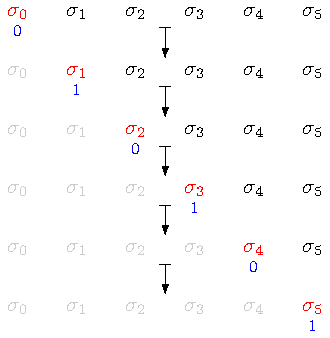
\includegraphics{figures/parity-checker.pdf}
  \caption{An illustration of the process. In each step, gray
    represents characters that've already been read, red symbols
    represent the current character, and blue symbol indicate the
    value of the parity bit. The final parity is odd, so we reject.}
  \label{fig:illustration-of-process}
\end{figure}
We note that a computer built to execute this algorithm could be very
simple: it would only need enough memory to store the program and keep
track of the parity bit, and this would be sufficient to determine
membership in $L_{\rm easy}$ for arbitrary input.

By contrast, $L_{\rm hard}$ seems a lot harder. Since the input can be
made arbitrarily long\footnote{See: this document} while still
remaining valid,\footnote{See: maybe a different document} we need to
be able to keep track of claims that are made arbitrarily far apart in
the input string. E.g., suppose we're handed something like the
following:
\begin{itemize}
  \item Axioms: $A_0$, $A_1$, \ldots, $A_n$.
  \item Desired result: $Z$.
  \item Proof:
    \begin{itemize}
      \item $1 + 1 = 2$
      % \item $2 = 2$
      \item $1 + 2 = 3$
      \item (A bunch of \np{other statements that are true but
        irrelevant} interspersed randomly with helpful ones, until
        finally)
      \item $\ldots \implies Z$.
    \end{itemize}
\end{itemize}
A priori, a verifier program has no knowledge of which claims will be
relevant later to the proof. Hence, it needs to store all of the ones
it encounters --- even silly things like $1+1 = 2$. This makes it
impossible to create an algorithm that looks exclusively at local data
to verify whether a given string $\sigma \in L_{\rm hard}$. Thus, we
would need a more sophisticated computer to execute a verifier for
$L_{\rm hard}$ than we did for $L_{\rm easy}$.


This difference is made formal by the \emph{Chomsky Hierarchy}, which
gives an ordering to languages based on the complexity of the
``computers'' needed to identify their strings.\footnote{Technically
  ``computer'' should be replaced with ``computational model,'' but
  the distinction isn't important for us today} The situation is
summarized by the following graphic:
\begin{figure}[H]
  \centering
  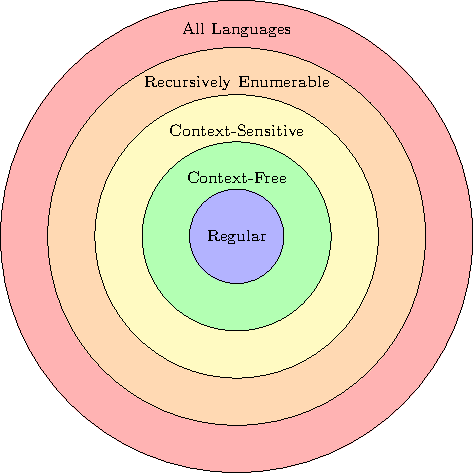
\includegraphics[scale=.8]{figures/chomsky-hierarchy.pdf}
  \caption{The Chomsky Hierarchy}
  \label{fig:chomsky-hierarchy}
\end{figure}
$L_{\rm easy}$ is a \emph{regular language}, which corresponds to one
of the simplest possible models of computation (a \emph{Deterministic
  Finite Automaton}). By contrast, $L_{\rm hard}$ requires a
\emph{Turing Machine}, one of the most powerful models of computation.
All of these can be unified into a single conceptual framework by
viewing them as \emph{dynamical systems}. The reader might consider
how as we begin with our formal definitions. But first, a quote from
Prof.\ Ran:
\begin{leftbar}
  ``There's this beautiful onion\ldots and if you cut it open, it will
  make you cry.''

  {\hfill\itshape -Prof.\ Ran, on the Chomsky Hierarchy}
\end{leftbar}
We will strive to ensure that the reader experiences only tears of
joy.


\subsection{Deterministic Finite Automata}
\emph{Deterministic finite automata} correspond to the innermost ring
of \cref{fig:chomsky-hierarchy}, the \emph{regular languages}. These
can be described formally in a number of ways; we'll choose the
following:
\begin{definition}[Regular Language]\label{def:regular-language}
  Let $\Sigma$ be an alphabet. We'll define the set of all
  \emph{regular languages over $\Sigma$} (denoted $\lreg(\Sigma)$) by
  an iterative process:
  \begin{enumerate}
    \item First, define $\varnothing$ and $\set{\epsilon}$ to be
      elements of $\lreg(\Sigma)$.
    \item Next: For all $\sigma \in \Sigma$, define $\set{\sigma}$ to
      be an element of $\lreg(\Sigma)$.
    \item Now, for all $L_0$, $L_1 \in \lreg(\Sigma)$, define
      \begin{itemize}
        \item $L_0 \cup L_1$, % {\color{red} (note, we allow only finite
          % unions)}
        \item $L_0 \cdot L_1 = \set{\ell_0 \ell_1 \MID \ell_0 \in L_0,
          \ell_1 \in L_1}$, and
        \item $L_0^\star$, $L_1^\star$
      \end{itemize}
      to be elements of $\lreg(\Sigma)$.
    \item Finally, if $L$ is yielded by a finite sequence of the
      rules above, then $L \in \lreg(\Sigma)$. \qedhere
  \end{enumerate}
\end{definition}
The idea with regular languages is that they are only slightly more
complicated than $\Sigma$ itself. Indeed, one might note the
similarity between the axioms above and those for \cref{def:strings}
(strings). We'll give a few examples of regular languages before we
introduce the associated model of computation. To that end, we'll
first introduce a shorthand that will reappear many times throughout
this paper.
\begin{definition}[Exponent notation]
  Let $\Sigma$ be an alphabet. Then for all $\sigma \in \Sigma$, we
  interpret the notation $\sigma^n$ by
  \[
    \sigma^n = \underbrace{\sigma \cdot \sigma \cdots \sigma}_{n\text{
      times}} \qedhere
  \]
\end{definition}
In light of the remark about {\color{red} m} {\color{orange} o}
{\color{yellow} n} {\color{green} o} {\color{blue} i} {\color{purple}
  d}s made earlier, this notation is actually quite reasonable.
\begin{example}\label{ex:dfa-example}
  Let $\Sigma = \set{0,1}$. Then $L$ defined by
  \[
    L = \set{0^n 1^m \MID n,m \in \NN}
  \]
  is a regular language. This follows from the fact that we can write
  $L$ as $L = \set{0}^\star \cdot \set{1}^\star$.
\end{example}
\begin{example}
  Let $\Sigma$ be an arbitrary alphabet. Then all finite sets $L
  \subseteq \Sigma$ are regular. This follows from the fact that for
  any $\sigma\in L$, if $\sigma$ decomposes as
  \[
    \sigma = \sigma_{i_1} \sigma_{i_2} \cdots \sigma_{i_k},
  \]
  Then we can state this equivalently as
  \[
    \set{\sigma} = \set{\sigma_{i_1}} \cdot \set{\sigma_{i_2}} \cdots
    \set{\sigma_{i_k}},
  \]
  from which it follows that $\set{\sigma}$ is regular. Finally, this
  gives us that
  \[
    L = \bigcup_{\sigma \in L} \set{\sigma}
  \]
  is a regular language.
\end{example}
\begin{example}
  Let $\Sigma = \set{0,1}$. Then $L$ given by $L = \set{(01)^n \MID n
    \in \NN}$ is regular.
\end{example}
As stated earlier, \emph{regular languages} are tied to
\emph{Deterministic Finite Automata}. These will lead to a more
dynamical systems-esque view of regular languages.
\begin{definition}[Deterministic Finite Automata]
  A \emph{deterministic finite automata} is a 5-tuple
  \[
    M = (Q, F, \Sigma, \delta, q_0)
  \]
  such that the following hold:
  \begin{enumerate}
    \item $Q$, $\Sigma$, $F$ are finite sets. We choose the following
      naming conventions:
      \begin{enumerate}[label=\roman*)]
        \item $Q$ is called the \emph{set of states} for $M$,
        \item $F$ is called the set of \emph{accepting} states for
          $M$, and
        \item $\Sigma$ is called the \emph{input alphabet} for $M$;
      \end{enumerate}
    \item $\delta$ is a function $\delta : Q \times \Sigma \to Q$ (we
      call $\delta$ the \emph{transition function}), and
    \item $q_0 \in Q$ is a distinguished element that we call the
      \emph{start state}. \qedhere
  \end{enumerate}
\end{definition}
We imagine $M$ performing a computation as follows: Suppose we're
given an input string $\sigma = \sigma_{i_1} \sigma_{i_2} \ldots
\sigma_{i_k}$. $M$ initializes in the \emph{start state} $q_0$, and
reads the first character. $M$ then changes state to $q_{j_1} =
\delta(q_0, \sigma_{i_1})$, and reads the next character
$\sigma_{i_2}$. $M$ then transitions to state $q_{j_2} =
\delta(q_{j_1}, \sigma_{i_2})$, and so on. Once $M$ has exhausted the
input, it halts computation. If it halts in an \emph{accepting state}
(i.e.\ $q_{\rm final} \in F$), then we say $M$ accepts the input;
else, we say $M$ rejects it.

It's common to visualize DFAs through diagrams like the following:
\begin{figure}[H]
  \centering
  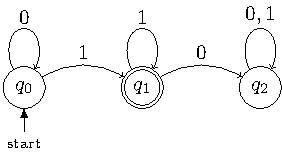
\includegraphics[scale=1.2]{figures/dfa-example.pdf}
  \caption{A DFA for \cref{ex:dfa-example}.}
\end{figure}
The common convention is that circles represent states of $Q$; the
arrows represent the transitions given by $\delta(q, \sigma)$ (where
$\sigma$ is the label above the arrow), and double-circled states
represent elements of $F$.




\subsection{}








% {\color{blue} helkjjjjsdf;af}






\subsection{Turing Machines}
A \emph{Turing machine} (often TM for short) is an abstract model of
computation that allows us to encode computer programs as collections
of sets with well-defined maps. There are many ``equivalent''
definitions for Turing machines;\footnote{Here, ``equivalent'' means
  that the models of computation they define are equally powerful.
  That is, given two distinct definitions $D_0, D_1$ for Turing
  machines, the behavior of any machine defined with $D_0$ can be
  simulated using a machine defined by $D_1$ and vice versa.} we'll
give the canonical one first and save the more
dynamical-systems-flavored version for later.
\begin{definition}[Turing Machine]
  A \emph{Turing machine} is a {\color{red} 5}-tuple
  \[
    M = \pn{Q, F, \Gamma, \Sigma, \delta}
  \]
  such that the following conditions hold:
  \begin{enumerate}[label=\arabic*)]
    \item $Q, F, \Gamma, \Sigma$ and $F$ are finite sets. Note, we
      choose the following naming conventions:
      \begin{enumerate}[label=\roman*)]
        \item $Q$ is called the set of \emph{states} for $M$,
        \item $F = \set{\cmark, \xmark}$ is called the set of
          \emph{final states} (read ``accept'' and ``reject''
          respectively),
        \item $\Gamma$ is called the \emph{work alphabet}, and
        \item $\Sigma$ is called the \emph{input alphabet};
      \end{enumerate}
    \item $F \subseteq Q$ and $\Sigma \subseteq \Gamma$;
    \item $Q$ contains a distinguished element $q_0$, called the
      \emph{start state} or \emph{initial state};
    \item $\Gamma$ contains a distinguished element $\blank$ called the
      \emph{blank character} (we require $\blank \not \in \Sigma$);
    \item $\delta$ (called the \emph{transition function}) has the
      following properties:
      \begin{enumerate}[label=\roman*)]
        \item $\delta$ is a partial function $\delta : (Q \setminus F)
          \times \Gamma \nrightarrow Q \times \Gamma \times
          \set{L,R}$. Note the inclusion of the word \emph{partial}
          --- in general we do not require $\delta$ to be defined on
          all of $(Q \setminus F) \times \Gamma$.
        \item $L, R$ are understood as ``shift'' directions, as
          explained below. \qedhere
      \end{enumerate}
  \end{enumerate}
\end{definition}
We think of Turing machines as operating on an infinite \emph{work
  tape}, where the cells of the tape each represent a symbol from the
alphabet $\Gamma$.\footnote{Formally, the addition of the tape
  requires using an infinite tuple of elements from
  $\prod_{i=-\infty}^\infty \Gamma$, with all but finitely-many
  entries non-blank.} One can think of this tape as representing the
``memory'' of the TM.

The tape is initialized with a finite word $\sigma = \sigma_1 \sigma_2
\cdots \sigma_n$ representing the input to our program, while the rest
of the tape is filled with $\blank$ characters. The TM initializes in
the \emph{start state}, with the \emph{tape head} (drawn with an
$\uparrow$ in the below) on $\sigma_1$. We think of the tape head as
``pointing'' to whatever character the TM is reading currently.
\begin{figure}[H]
  \centering
  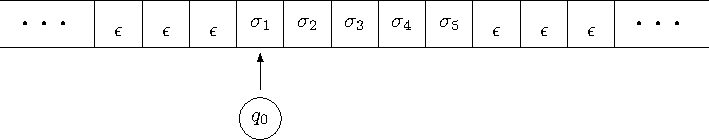
\includegraphics[scale=.7]{figures/tm-initial-input.pdf}
  \caption{Turing machine initialized with the input string $\sigma_1
    \sigma_2 \sigma_3 \sigma_4 \sigma_5$.}
\end{figure}
The ``program'' is then executed by the $\delta$ function. For
instance, suppose $\delta(q_0, \sigma_1) = (q_i, \gamma_1, R)$. Then
we interpret this as the Turing machine writing a $\gamma_1$ on the
current tape, updating its state to $q_1$, and moving one space to the
right on the tape.
\begin{figure}[H]
  \centering
  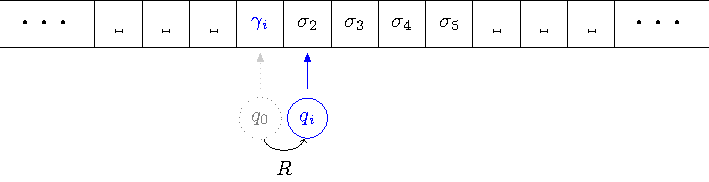
\includegraphics{figures/tm-one-step-later.pdf}
  \caption{Turing machine after performing a single step. Differences
    shown in {\color{blue} blue}.}
\end{figure}
At each step of the computation, the Turing machine performs a similar
process: Read the tape, rewrite and move as dictated by $\delta$, and
then repeat. If the Turing machine reaches the state $\cmark$, then it
halts and the input is said to be ``accepted.'' If it reaches
$\xmark$, the state is ``rejected.'' {\color{blue} In the case that
  the machine never halts, we treat this as a form of rejection.}



\section{Computational Universality}

A Universal Turing Machine is a Turing machine which can simulate any
arbitrary Turing Machine. It takes as its Turing Machine code, and an
input word, and then simulates the Turing Machine on that input.
Intuitively, any modern computer is a (finite memory) Universal Turing
Machine: it can store arbitrary computer programs as data, and then
run them on other data it stores or with user input.

In a similar vein, a system is {\it computationally universal} (or
just {\it universal}) if it has the ability to simulate an arbitrary
Turing machine. This is a loose definition because it is not
immediately clear what it means for a dynamical system to simulate a
Turing machine. There are many possible ways to create a more precise
definition; we will follow the method of Delvenne et al. [CITATION].
Before we do, though, we note a few reasonable expectations about what
simulating a Turing machine should mean:

\begin{itemize}
  \item If a dynamical system can simulate an arbitrary Turing machine, we should be able to take any combination of Turing machine and input, and convert it into some question about the system. The question should be ``equivalent'' to the question of whether the Turing machine would accept its input, in the sense that it should have a ``yes'' answer if the Turing machine accepts, and a ``no'' answer if the Turing machine rejects or never halts.

  \item The Universal Turing Machine is a specific Turing Machine that exists, and therefore it is a dynamical system on the space of its possible configurations. We would definitely expect this dynamical system to be considered universal.

  \item There are a number of other computational models which have ability to simulate Turing Machines, and which can also be considered dynamical systems. One good example is cellular automata, which are like Turing machine tapes where every cell has its own state and updates itself based on its neighbors' states. If a given instance of a computation model is capable of simulating arbitrary Turing machines, we would expect its associated dynamical system to be universal.

\end{itemize}

\subsection*{Formally defining universality}

We will follow the lead of Delvenne et al. [CITATION] in defining what
it means for a dynamical system to be universal. Like them, we will
consider only {\it symbolic} dynamical systems, that is, dynamical
systems on spaces consisting of infinite words made out of symbols
drawn from a finite alphabet. We will need to do some spadework before
we're ready to give the full definition.

\subsubsection*{Spadework Part I - R.E.-completeness}

Our ultimate goal is, given the code for a Turing machine $M$, and the
input $w$, to ask a question about a particular dynamical system which
has a ``yes'' answer exactly when $M$ accepts $w$. In the terms used
in the field of computability, we want to be able to reduce an
arbitrary instance of the question ``Will Turing machine $M$ accept
the input $w$?'' to a question about the dynamical system.

Fortunately, much is already known about the question ``Will Turing
machine $M$ accept the input $w$?''. In particular, it is equivalent
to the question ``Will Turing machine $M$ halt on the input $w$?'' in
the sense that if we had a way to answer either of the questions, we
could easily answer the other as well. This second question is called
the Halting Problem, and computer scientists say that it is ``complete
for the class of recursively enumerable problems.''

So, depending on your background, you may be asking two questions:
``What is the class of recursively enumberable problems?'' and ``What
does it mean to be complete for it?'' A problem is called recursively
enumerable if it can be solved by a Turing machine that may not ever
halt, that is, if the question has a ``yes'' answer, the Turing
machine will accept in finite time, but if the question has a ``no''
answer, the machine may run indefinitely. They are called
``recursively enumerable'' because it would be possible for a Turing
machine (a computation model capable of {\it recursion}) to {\it
  enumerate} every input that would have a ``yes'' answer, in such a
way that every such input would eventually be listed in finite time.
(The machine could do this by listing all inputs lexicographically,
and spending half its time simulating the computation on the first
input, a quarter of its time on the second input, and so on, printing
out any input when it is accepted.)

A given problem, call it $P$, is complete for a class of problems,
$C$, if two conditions hold. First, $P$ must be an element of $C$.
Second, all problems in $C$ must be reducible to $P$, meaning that if
$P' \in C$, we can convert any instance of $P'$ to an instance of $P$
that will have the same answer, without doing an unreasonable amount
of work in the conversion (for our purposes here, any finite
computation time is reasonable). The Halting Problem is known to be
complete for the recursively enumerable problems, or r.e.-complete.

The question ``Will Turing machine $M$ accept input $w$?'' (call it
$Q$) is also r.e.-complete. Recall that our goal was to find a
question $QDS$ about a dynamical system, which we could reduce $Q$ to.
One way to express this constraint is that $QDS$ should be
r.e.-complete: then both $QDS$ and $Q$ could be reduced to each other,
so they would be equivalent questions, which is what we are looking
for. In fact, we will see that the r.e.-completeness of $QDS$ is
exactly what we will require.

\subsubsection*{Spadework Part II - Effective Symbolic Systems}

A symbolic set can be thought of as a set of words made from a finite alphabet $A$. We could express such a set as $(A \cup \{B\})^\Nn$, meaning the set of one-sided infinite words with characters which are either drawn from $A$ or are the ``blank'' symbol $B$. Finite words would then end be expressed as infinite words ending with an infinite tail of $B$s. But we could encode each element of $A \cup \{B\}$ with a binary sequence (with all encodings the same length), so any symbolic set can be encoded as a subset of the set $\{0,1\}^\Nn$ of one-sided infinite binary words.

We give $\{0,1\}^\Nn$ the following distance metric $d$: $d(x,y) = 0$ if $x$ and $y$ agree at all indices, and otherwise $d(x,y) = 2^{-n}$ where $n$ is the smallest index at which $x$ and $y$ differ. Under this metric, the set of all sequences beginning with a finite binary word $w$ is a both a closed and open set (a ``clopen'' set) under this metric. Call sets like this, generated by a common prefix, cylinders. It can be shown that the clopen sets of $\{0,1\}^\Nn$ are precisely the finite unions of cylinders. What is special about this is that we can associate with each clopen subset of $\{0,1\}^\Nn$ a unique finite set of finite words, which are the generating prefixes for the cylinders that make up that set. So we can express every clopen set of $\{0,1\}^\Nn$ in a finite way, which means the we can list off all the clopen sets in some lexicographic order (in other words, the set is countable). We'll be exploiting this fact later.

Now we're ready to define the main dynamical systems we'll be working with. If $X \subseteq \{0,1\}^\Nn$ is a symbolic set and $f: X \to X$ is a continuous map on $X$, then $(X, f)$ is an {\it effective symbolic system} if:
\begin{enumerate}[label=(\roman*)]
  \item $X$ is closed.
  \item Checking whether some clopen set $Y \subseteq \{0,1\}^\Nn$ has a non-zero intersection with $X$ is decidable by a Turing machine in finite time.
  \item The inverse map $f^{-1}$ on clopen sets of $X$ can be computed in finite time.
\end{enumerate}

These requirements may seem a bit arbitrary, but they are made for a good reason. We will shortly be performing some operations on the clopen sets of $X$, and it turns out that, since $X$ is closed, these are exactly the intersections of $X$ with the clopen sets of $\{0,1\}^\Nn$, so we know this is a countable set. Requirement (ii) helps ensure that a Turing machine could list out these clopen sets without ever getting stuck checking if a particular clopen set of $\{0,1\}^\Nn$ has a nonempty intersection with $X$. And requirement (iii) foreshadows operations we will be doing on clopen sets.

\subsubsection*{Spadework Part III - Temporal Logic}

Recall that we are looking for a way to ``ask questions'' about dynamical systems, whose answers will tell us something about the behavior of Turing machines. In order to be able to construct such questions, we will use subsets of state space to encode logical statements. Since we want to be able to make statements about the {\it eventual} behavior of the system, we will use a logical framework called temporal logic. Temporal logic includes all of the standard logical operators:
\begin{itemize}
  \item $\top$: always true
  \item $\bot$: always false
  \item $\lor$: or
  \item $\lnot$: not
  \item $\land$: and (which is actually redundant because it is constructible from $\lor$ and $\lnot$)
\end{itemize}
It adds two additional operators to the list:
\begin{itemize}
  \item $\lnext$: next, a unary operator, with $\lnext \phi$ meaning that $\phi$ will be true after one time step.
  \item $\ltil$: until, a binary operator, with $\phi \ltil \psi$ meaning that $\psi$ will be true within finite time, and for all time between the present and one step before the time when $\psi$ is true (inclusive), $\phi$ will be true
\end{itemize}

The developers of temporal logic, Arthur Prior and Hans Kamp, have described a set of rules for incorporating these operators into classical logic in a way that is consistent with our interpretation of them [CITATION]. For our purposes, suffice it to say that it works.

How do we propose to use temporal logic to construct statements about effective symbolic systems? Well, as we have suggested above, we are interested in operating on the clopen sets of symbolic systems, and here is where that will come into play. Let's say we have some effective dynamical system $(X, f)$. We will use the fact that the clopen subsets of $X$ are countable, and let $P_0, P_1, P_2, ...$ be a listing of all the clopen subsets of $X$ (including $\emptyset$ and $X$ in some positions).

Then let $\psc_0, \psc_1, \psc_2, ...$ be a set of propositional symbols, which are the logical ``units'' that along with the operators above are the building blocks of temporal logic formulas. The listing will contain $\top$ and $\bot$ in some positions. We're going to define an ``interpretation'' operator $\abs{\cdot}$ that takes logical formulas to subsets of $X$. The intuition behind it will be that if $\phi$ is a logical formula that expresses something about the ``current configuration of the system,'' $|\phi|$ is the set of possible system configurations (points of $X$) for which that statement is true. Formally, the operator will behave like this:

\begin{itemize}
  \item If $\phi$ is just the symbol $\psc_n$, $\abs{\phi} = P_n$, and we stipulate that the orderings should align such that $\abs{\top} = X$ and $\abs{\bot} = \emptyset$. This means that the symbol $\psc_n$ represents the statement ``The current system configuration is in the set $P_n$,'' which is of course always true if $P_n = X$ and never true if $P_n = \emptyset$.

  \item $\abs{\phi_1 \lor \phi_2} = \abs{\phi_1} \cup \abs{\phi_2}$, because for either $\phi_1$ or $\phi_2$ to be true, the system can be in any state in which either is true.

  \item $\abs{\lnot \phi} = X \setminus \abs{\phi}$, because the set of states for which $\phi$ is not true is the complement of the set of states for which it is.

  \item $\abs{\lnext \phi} = f^{-1}\left( \abs{\phi} \right)$, which means that $\lnext \phi$ represents the statement, $\phi$ will be true after one application of $f$, meaning that each application of $f$ corresponds to one ``time step'' within the temporal logic system. Note that we know that this is computable, by requirement (iii) of effective symbolic systems.

  \item $\abs{\phi_1 \ltil \phi_2} = \bigcup_{n \in \Nn} A_n$ with $A_0 = \abs{\phi_2}$ and the other sets defined by the recurrence relation $A_{n+1} = f^{-1}(A_n)\cap\abs{\phi_1}$. Here $A_n$ can be interpreted as, the set of system states for which $\phi_2$ will be true on the $n^{\text{th}}$ time step from the current state, and $\phi_1$ will be true on the $0,...n-1$ time steps. The union of all of these represents all states for which ``$\phi_1$ is true until $\phi_2$ is eventually true.''

    So, in short, we have used temporal logic to construct a set of formula that express statements about the state of the system. We say a given formula is satisfiable if its interpretation is non-empty, meaning that there is some nonempty set of $X$ that satisfies it.

\end{itemize}


\subsubsection*{Universality}

Our spadework concluded, we're ready to say what it means for an effective dynamical system to be universal. We will use Delvenne et. al's precise definition here:

``{\it An effective dynamical system is \emph{universal} if there is a recursive family of temporal formulae such that knowing whether a given formula of the family is satisfiable is an r.e.-complete problem.}''

A ``recursive'' family of temporal formulae is a set of temporal formula for which membership in the set can be decided by a turing machine in finite time; this is essentially a regularity condition which prevents the family from being outlandishly defined.

To get a feel for what this definition means, and ensure that it is reasonable, let's start by confirming that the Universal Turing Machine dynamical system  is, as we expected from the start, universal.

A configuration of the Universal Turing Machine, as with all Turing machines, is defined by finite control state and its tape contents, both of which can be encoded in a binary strings. So the configuration space of a UTM is a subset $X$ of $\{0,1\}^\Nn$, and the code for the UTM is some specific transition function on this space, $f$.
\end{multicols}
\end{document}
